\section{Image Processing}

To carry out the image processing we used very simple theoretical notions. The library we used is open cv. The figure below summarizes our image processing.
\begin{figure}[ht!]
    \begin{center}
        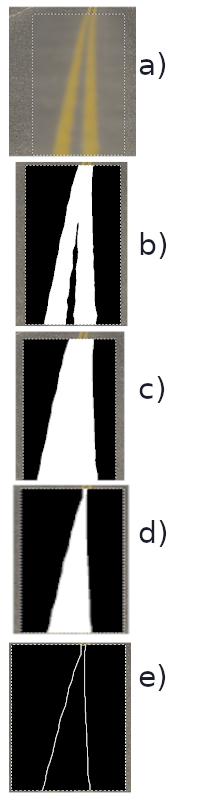
\includegraphics[scale=0.3]{Images/diagramme.png}
    \end{center}
    \caption{image processed}
    \label{fig:img_processing}
\end{figure}

\subsection{Data logging}
For the first part of this image processing, we had to collect images.
So first we went into the environment in which the robot was going to evolve.

\begin{figure}[ht!]
    \begin{center}
        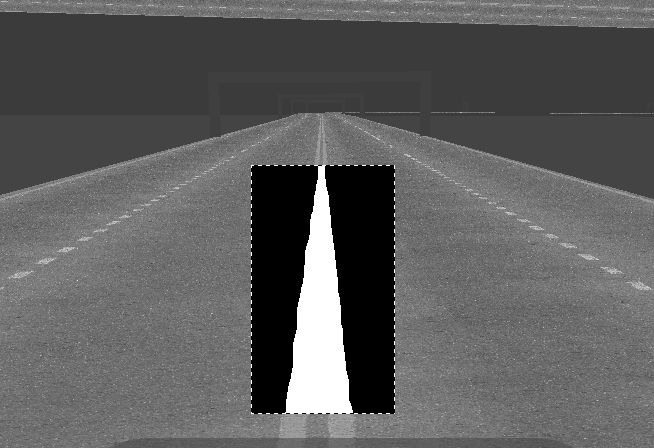
\includegraphics[scale=0.3]{Images/image_process.png}
    \end{center}
    \caption{image processed}
    \label{fig:img_processing}
\end{figure}

\subsection{Pre binarization treatment}
In this part, we first had to perform a pre-binarization treatment in order to reduce post-binarization noise.
So we used a Gaussian filter to blur the image.

\subsection{Binarization}
Since the line we wanted to mark is white. An effective treatment is simply to switch to grey level. 
So for binarization, we switch the image to a grey level and threshold for a grey level that we have determined empirically.

\subsection{Morphological treatment}
In this part we performed a morphological treatment. There was still a lot of noise after binarization. So we made an opening. 
With a kernel in the shape of a rectangle (since it was the most efficient for this treatment).
At the end of this treatment we obtain a well defined line which crosses the screen.

\subsection{Barycenter of the line}
In this last part, the contours are marked using a gradient method. Then the contours are sorted from the smallest to the largest.
We recover the largest contour.
And we recover the coordinates of the barycentre of the contour.
Then the error is the difference between the center of the image and the coordinates of the pixel.
The problem with this method is that with the barycentre we have a regulation on a point in the centre of the image. And therefore, we don't use all the data we have.
So we decided to use the highest points of the contour.
Indeed, the position of the center of the line at the highest point of the image gives us an idea of the evolution of the road at the moment. From now on we use the horizon. It allows us to get information further into the "future". And so it allows for better regulation and therefore to go faster.
